\chapter{Combined search for invisibly decaying Higgs bosons in hadronic channels}
\label{chap:higgstoinv}

\initial{P}articles that escape the detector unseen in any experiment make them, by design, notoriously difficult to search for. The Higgs boson is particularly troublesome with its small production rate at the \acrshort{lhc}, and a predicted branching ratio to invisible states to match. As described in Chpt.~\ref{sec:theory_higgs_to_inv}, the leading estimates are still far higher than the \acrlong{sm}'s value. For the best chance of observing this decay, the inclusion of all of the Higgs boson's production modes is a necessity.

%=======
\begin{easylist}[itemize]
    \easylistprops
    & Discuss how the theoretical aspects from the Theory chapter translate into an experimental search.

    & Discuss the necessity of including all production modes of Higgs (invisible final state, so characterise events based on initial/additional particles). Also mention how sensitive each production mode is at contributing to the branching ratio limit. Emphasize the non-VBF modes (\ggF, \ttH, \VH\ -- \WplusH, \WminusH, \ZH) in this chapter as that's what I've been working on and another group will be covering \acrshort{vbf}.

    & Add a section or subsection somewhere regarding analysis tools. Perhaps add a brief description of \ROOT (and how it's entrenched in HEP even though people are tending to move away from \ROOT-based analysis onto more industry-standard tools), then lead into the FAST tools and using dataframes, vectorisation, etc., with only small interfaces to \ROOT (for I/O) to extract data. Potentially mention how the data tiers work in CMS (RAW, DIGI, RECO, AOD, miniAOD, nanoAOD, etc.)

    & Include object definitions, overall analysis strategy, triggers, signal production (with each non-VBF mode in detail), event selection, background estimation (\glspl{CR}, \glspl{SB}) and results/limit (including comparisons to previous results).

    & Emphasize my contributions: control region construction and studies, background estimation, and other studies I will have conducted by the time I write up.

    & Current material: no public plots as of yet. Hope to finish analysis soon. We are preparing a CMS internal analysis note, documenting all aspects of the analysis. I will first add all relevant information there which I can subsequently use when writing this chapter.

    & Since it's my thesis, I can talk about \ttH, \VH and \ggF/monojet, even though the Bristol contribution to the final, public result would only be \ttH and resolved \VH. Would need to be able to run the fit for all three modes simultaneously, ensuring we have complete (and correct) systematics for \ggF.
\end{easylist}

% Can pull from Section 37 of my lab book, and all the talks I and other people from the team have given (Presentations and talks/ folder, also Other peoples/ subdirectory). Can also pull from AN for analysis strategy


%=========================================================


\section{Production modes of the Higgs boson}
\label{sec:htoinv_production_modes}

At the \acrshort{lhc}, the most common mechanisms for producing a Higgs boson are \acrfull{vbf}, gluon-gluon fusion (\ggF), associated production from top quarks (\ttH), and associated production from a vector boson (\VH). Feynman diagrams of these processes are shown in Fig.~\ref{fig:higgs_feynman_diagrams}. They have very different characteristics, production rates, and event signatures, complementing each other and allowing a single analysis to cover all bases with orthogonal parameter spaces to target the individually. \footnote{Expand on these --- what the final states are and how they can be detected (e.g., use \mjj for VBF), cross sections, etc., possibly with a separate paragraph for each mode.}

\begin{figure}[htbp]
    \centering
    \begin{subfigure}[b]{0.45\textwidth}
        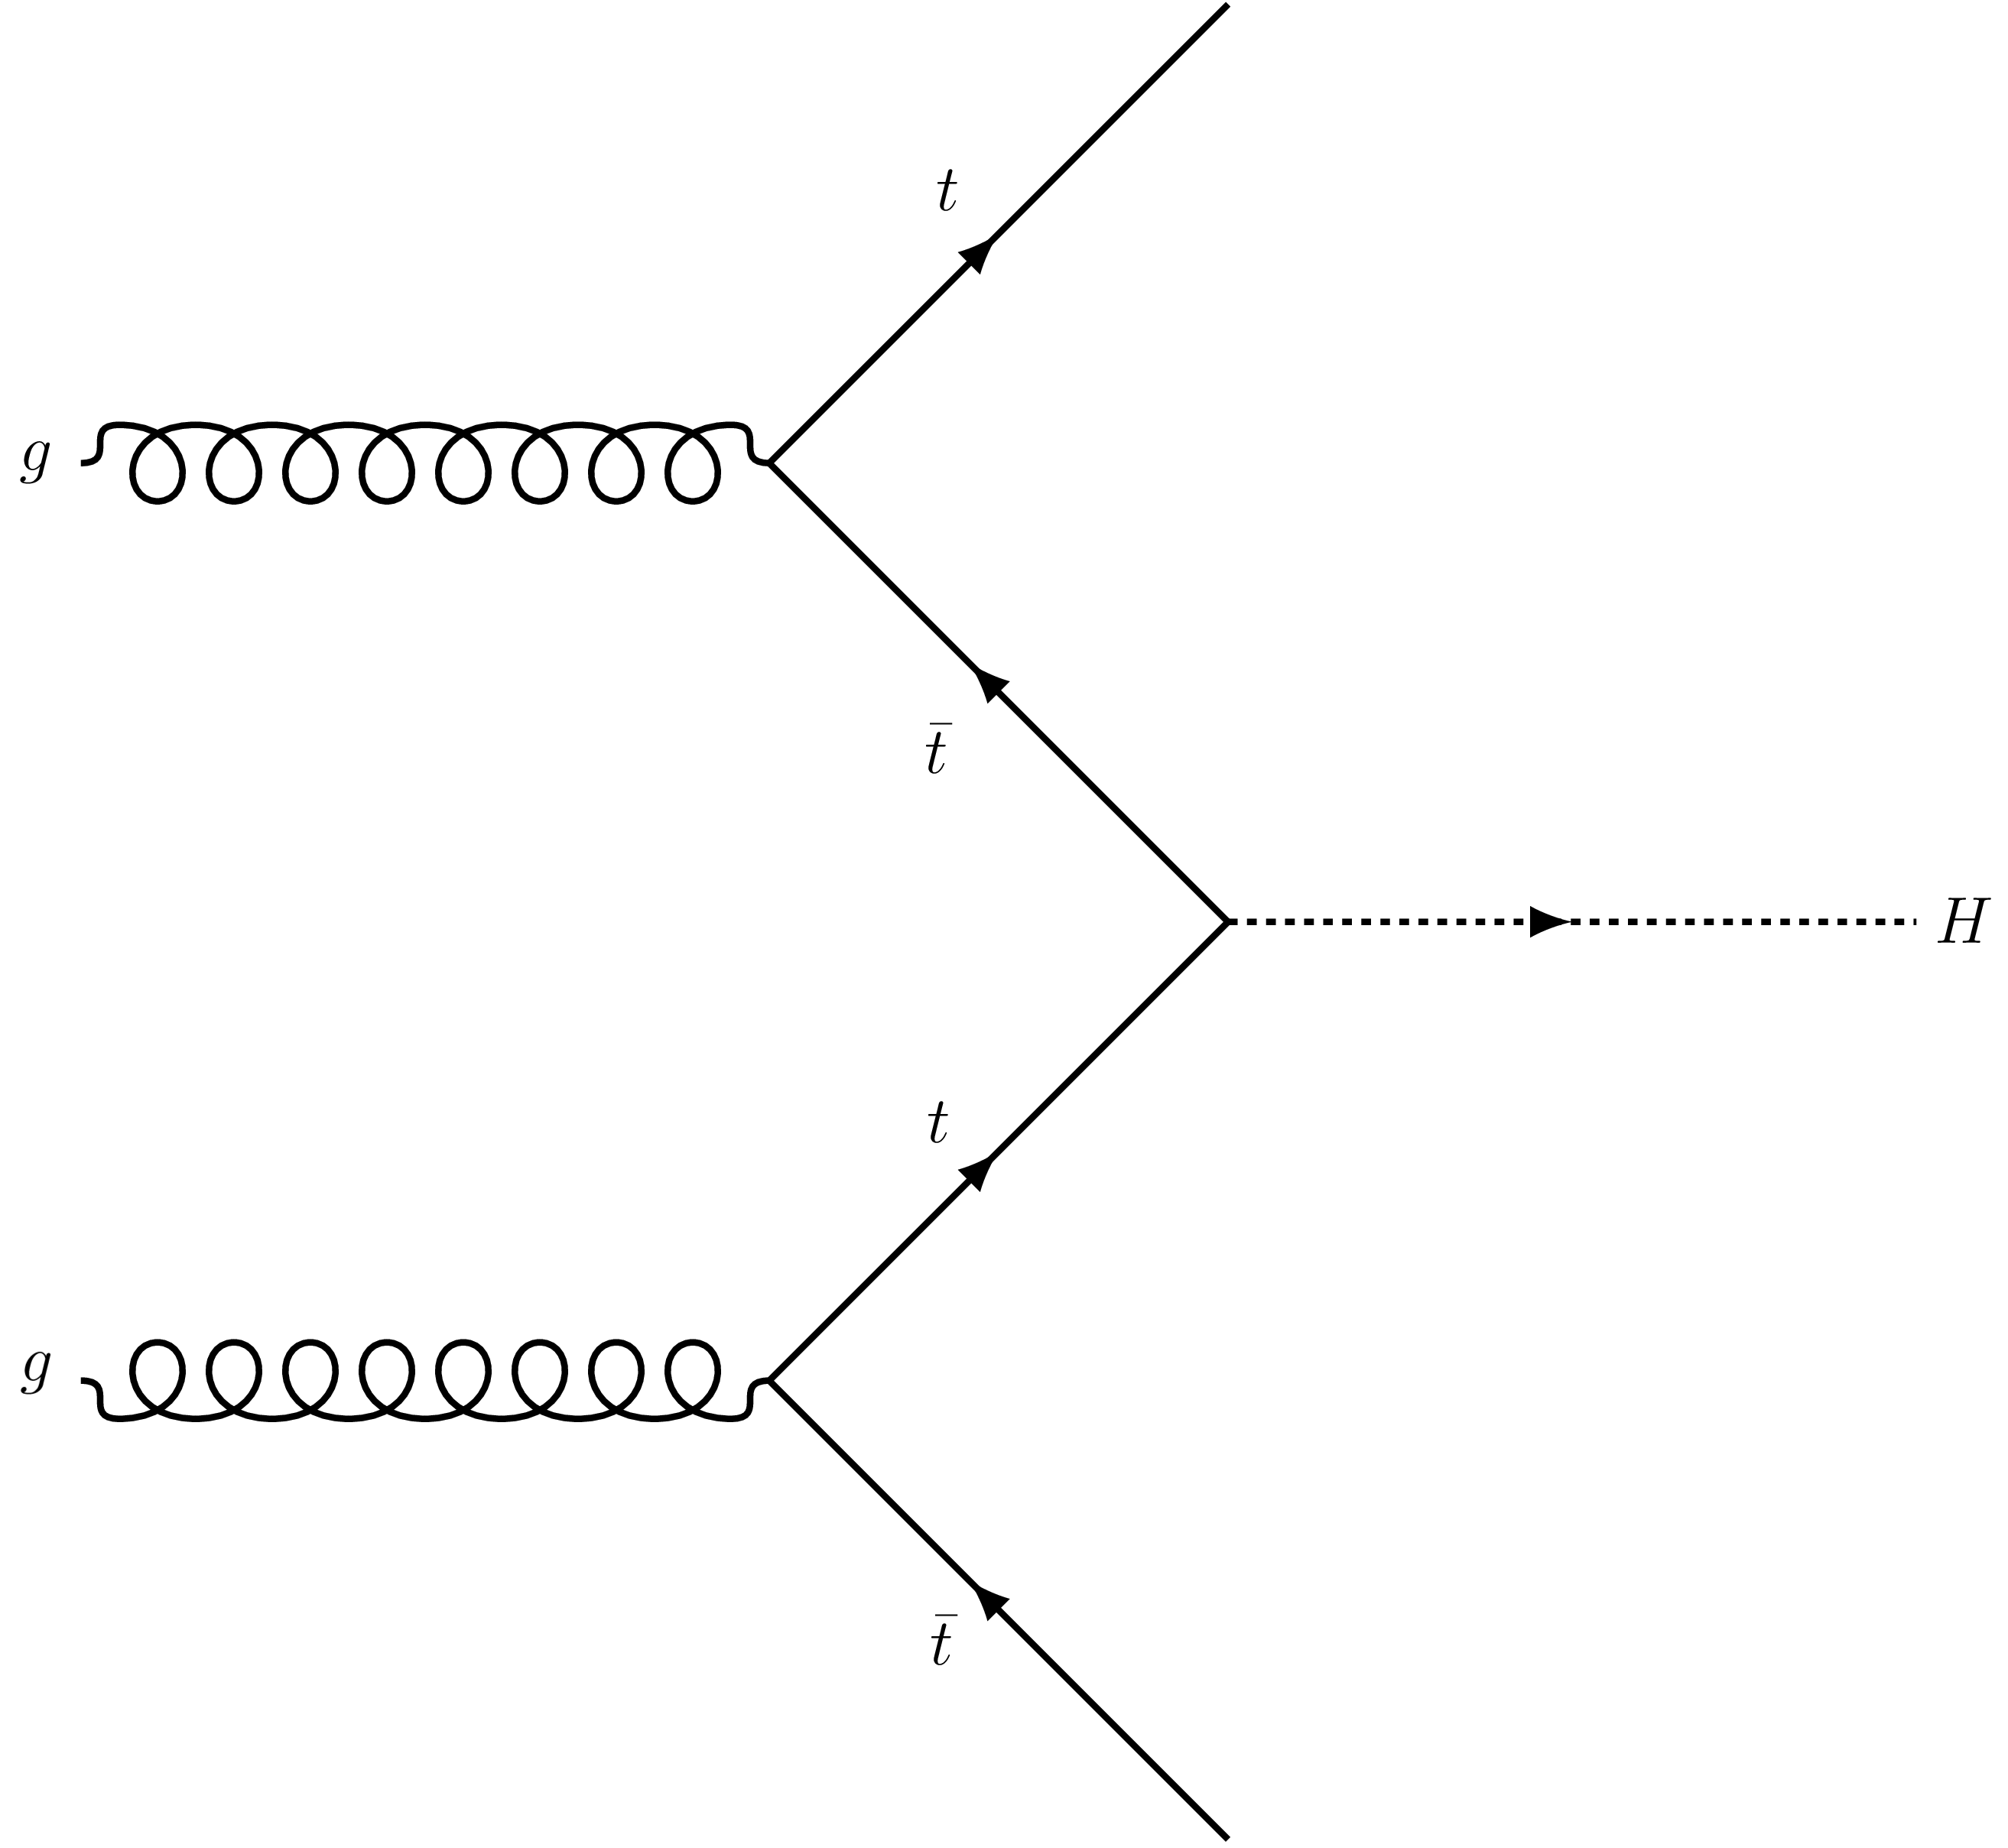
\includegraphics[width=\textwidth]{feynman_diagrams/ttH.png}
        \caption{\ttH}
    \end{subfigure}
    \hfill
    \begin{subfigure}[b]{0.45\textwidth}
        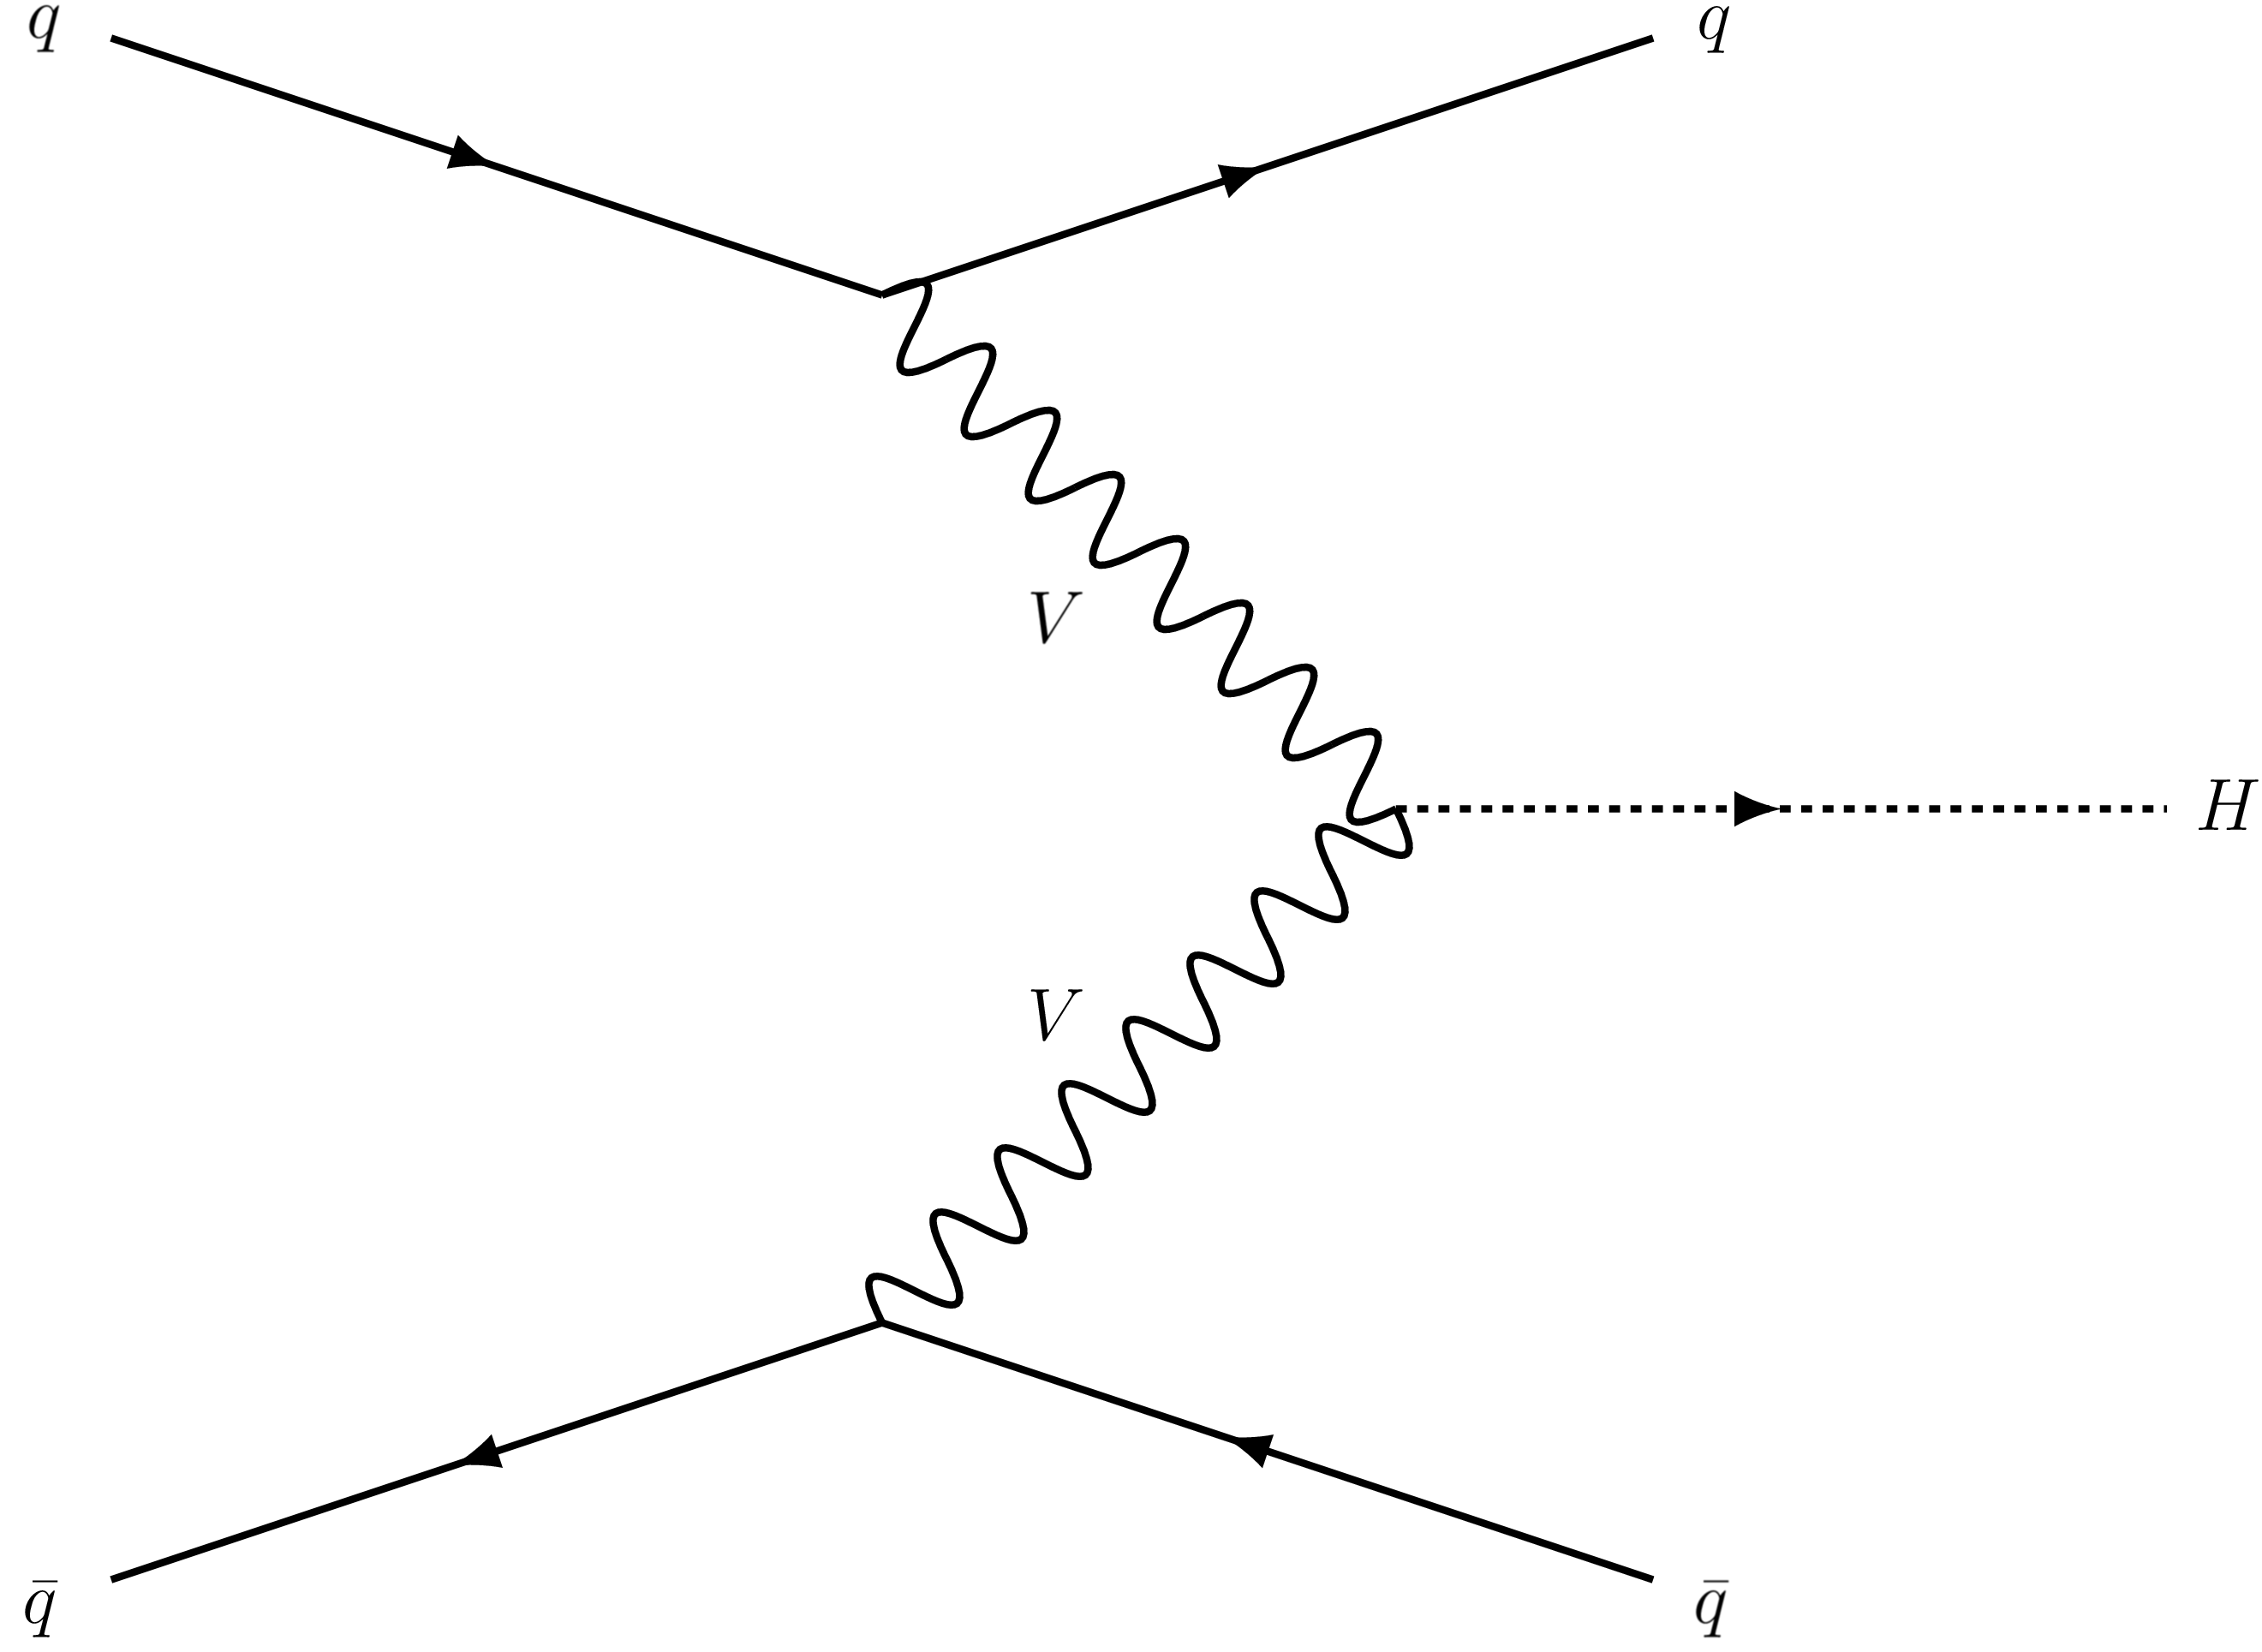
\includegraphics[width=\textwidth]{feynman_diagrams/VBF.png}
        \caption{\acrshort{vbf}}
    \end{subfigure}
% blank line to start new row
    \begin{subfigure}[b]{0.45\textwidth}
        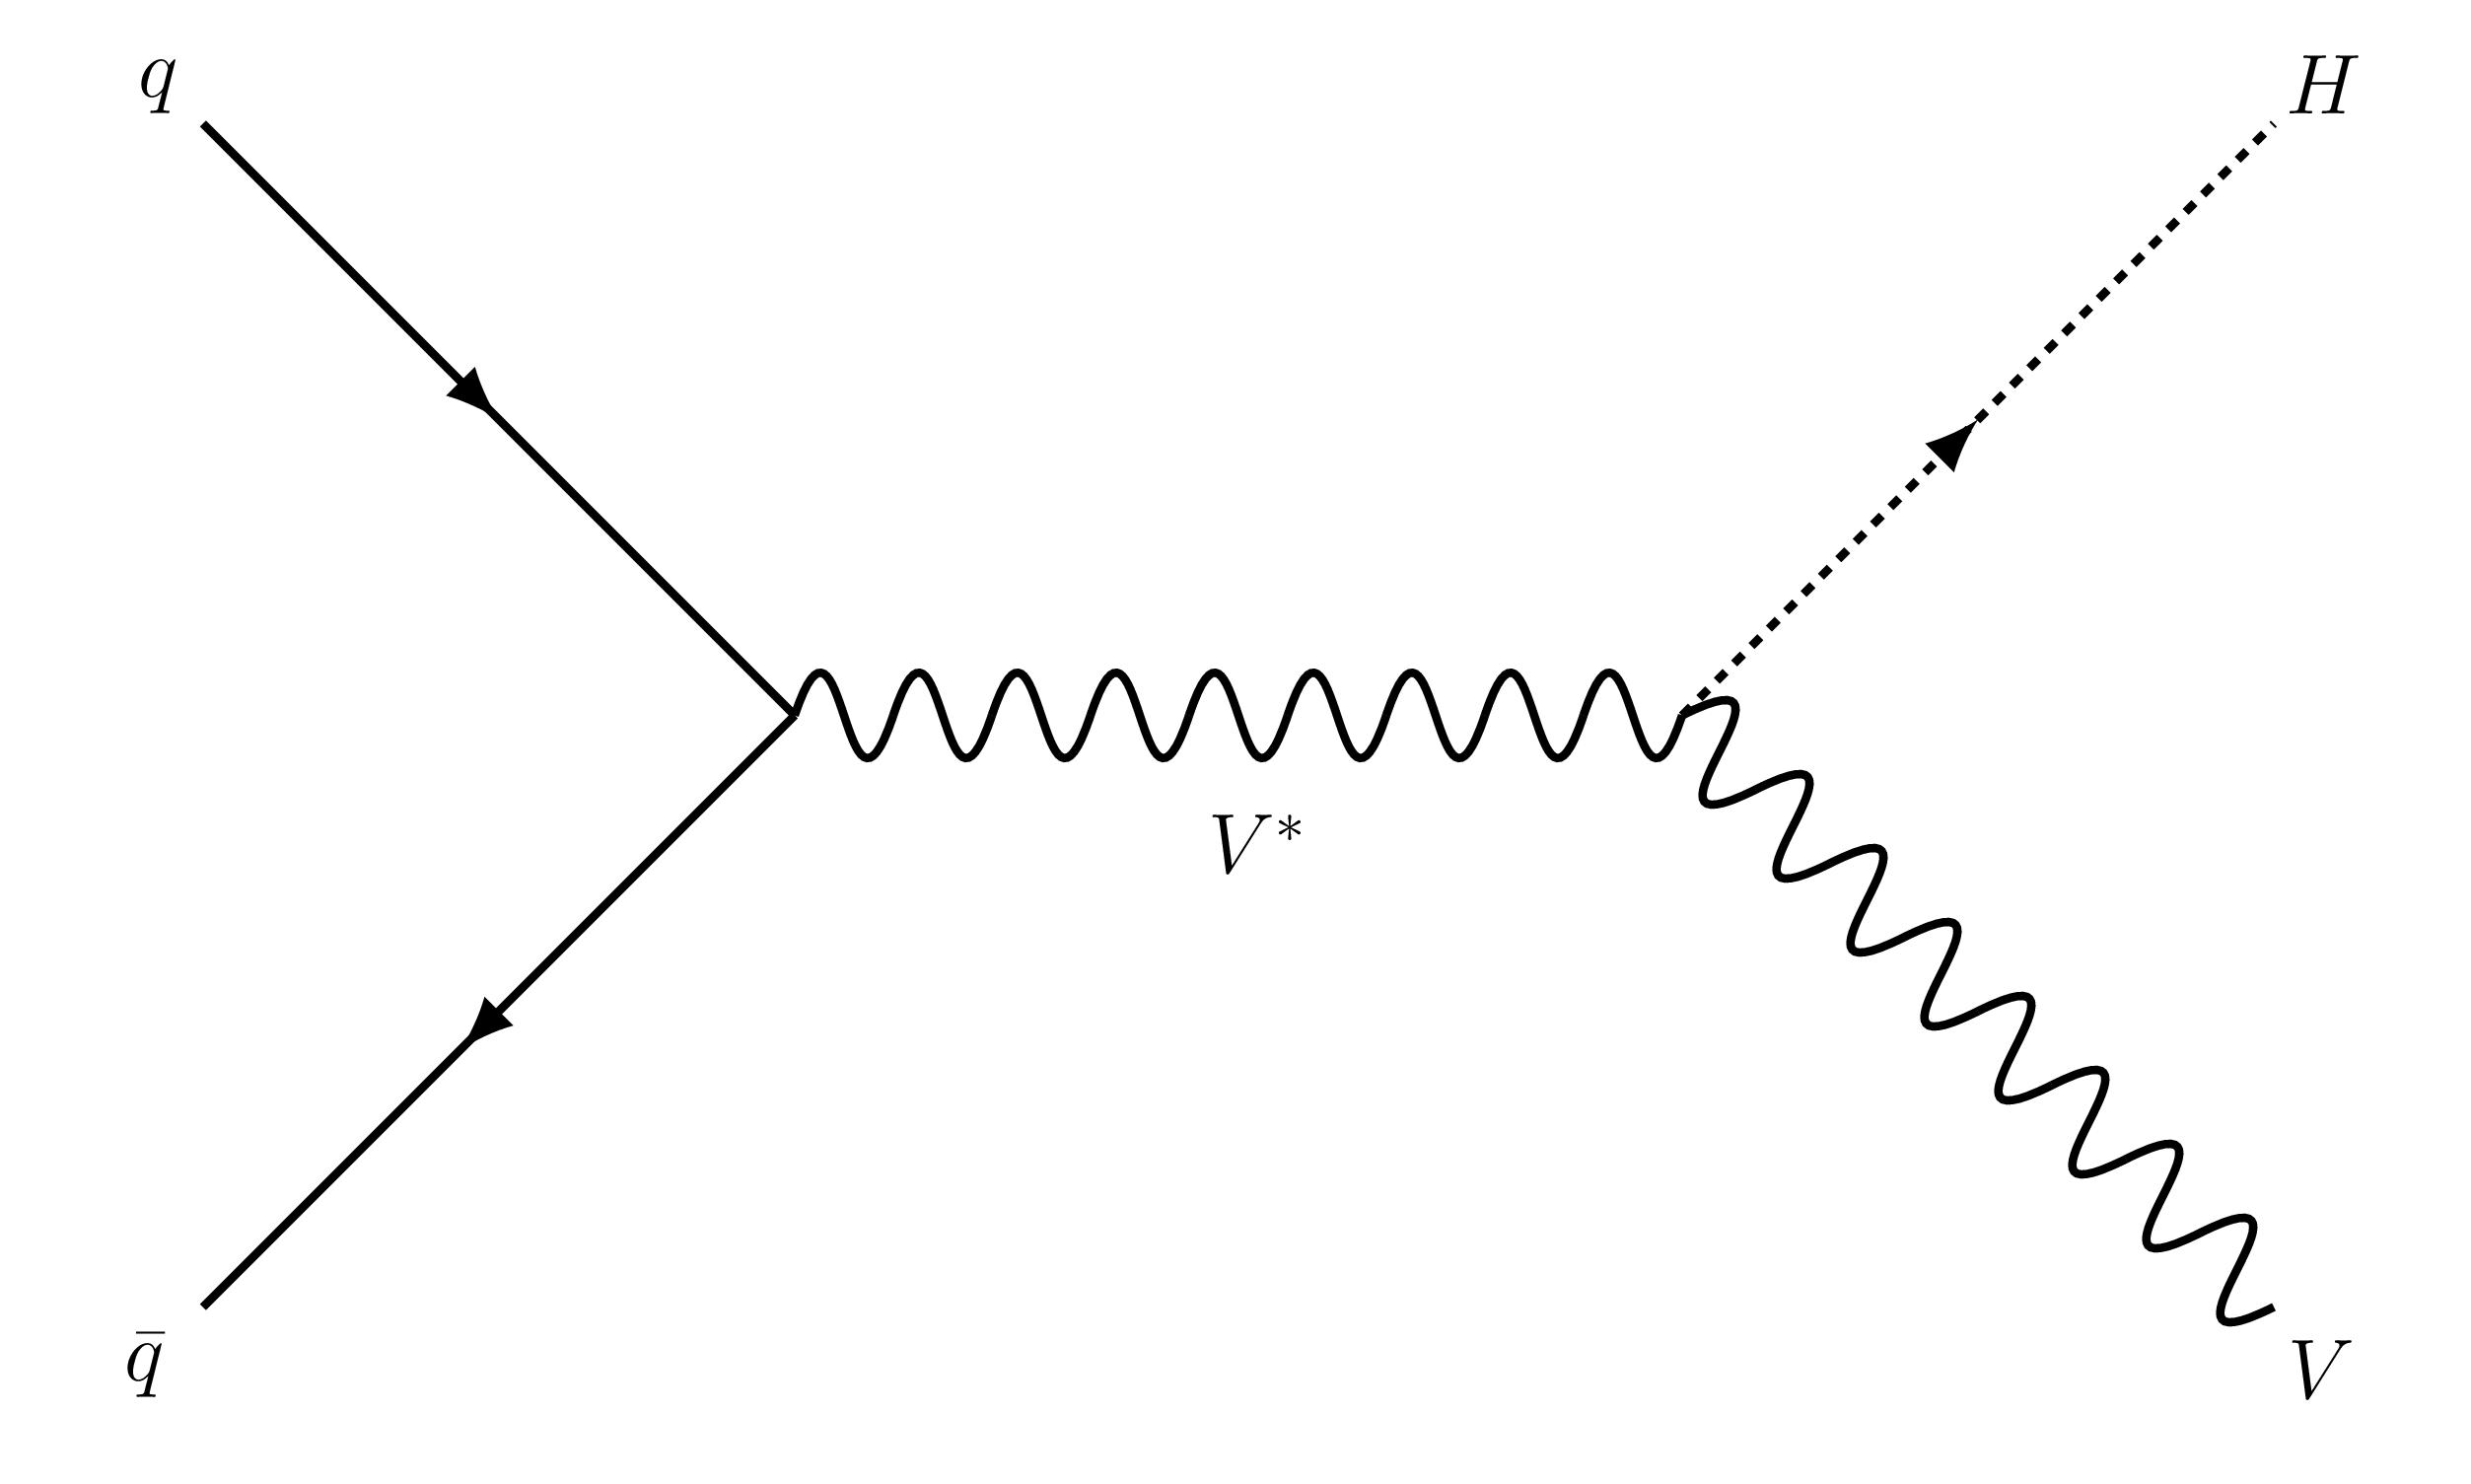
\includegraphics[width=\textwidth]{feynman_diagrams/VH.png}
        \caption{\VH}
    \end{subfigure}
    \hfill
    \begin{subfigure}[b]{0.45\textwidth}
        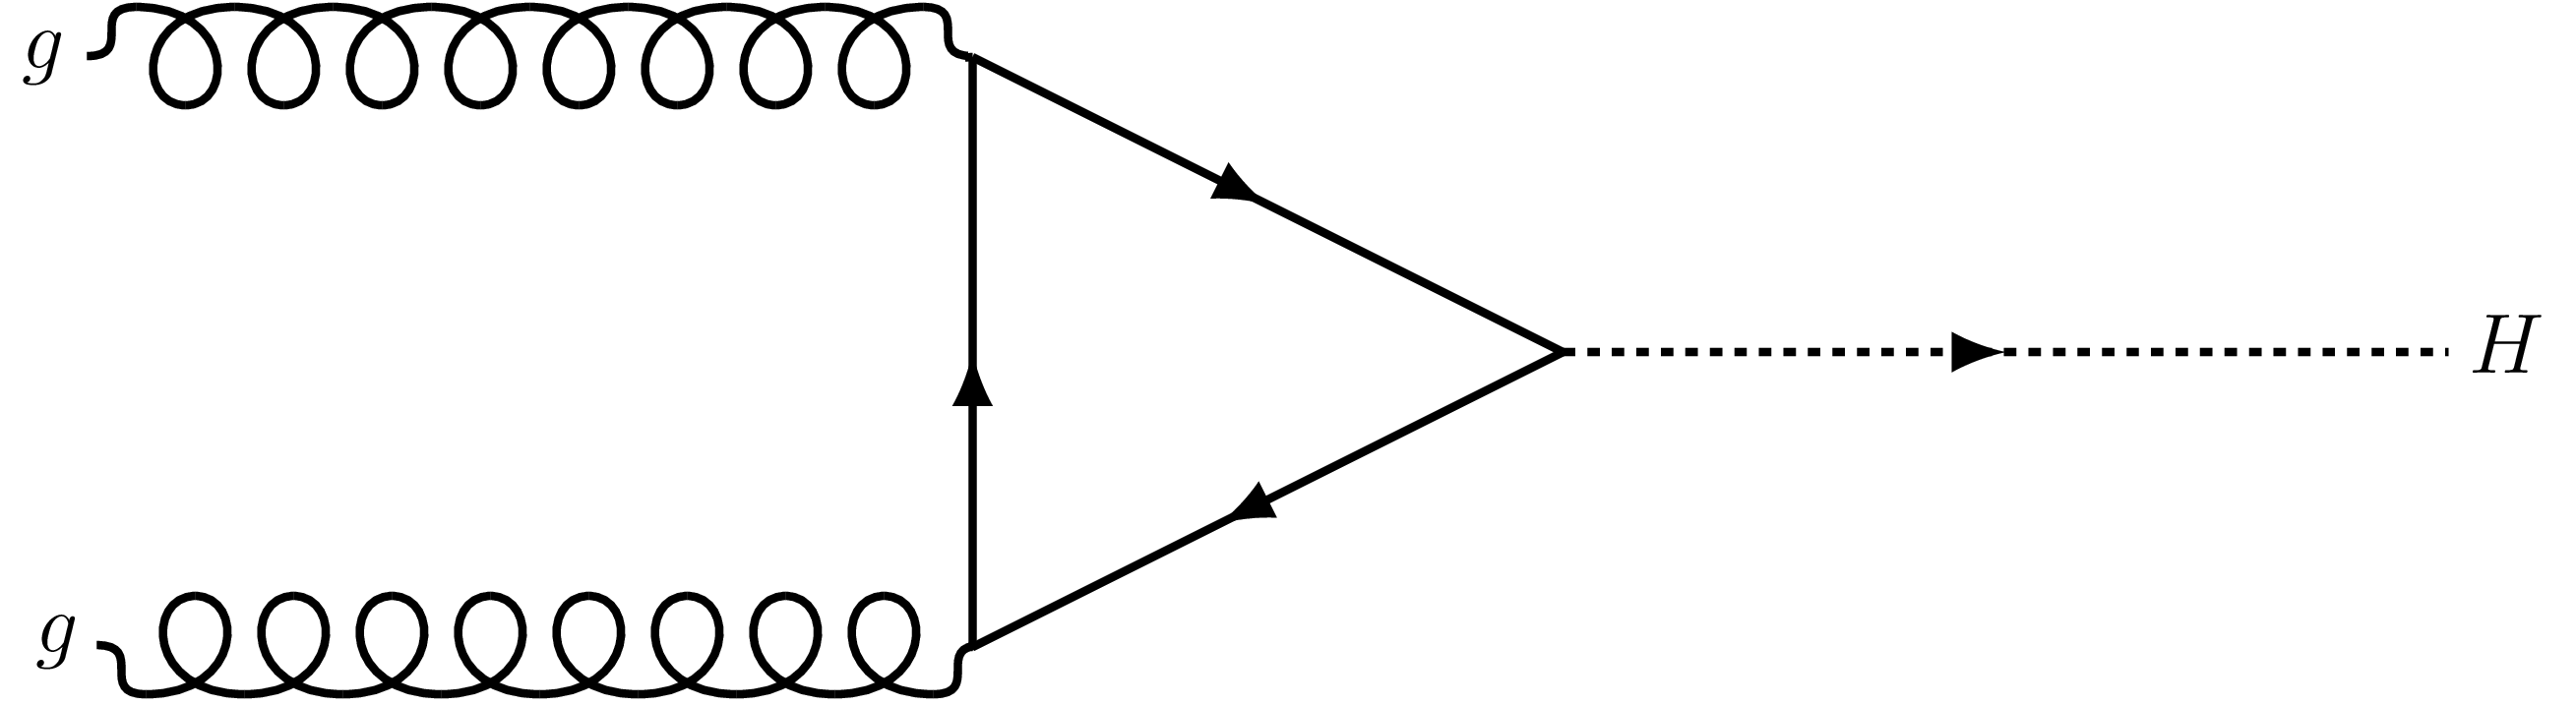
\includegraphics[width=\textwidth]{feynman_diagrams/ggF.png}
        \caption{\ggF}
    \end{subfigure}
\caption[The Feynman diagrams for the four predominant production mechanisms of the Higgs boson at the LHC]{The Feynman diagrams for the four predominant production mechanisms of the Higgs boson at the \acrshort{lhc}.}
\label{fig:higgs_feynman_diagrams}
\end{figure}


%=========================================================


\subsection{Vector boson fusion (VBF)}
\label{subsec:htoinv_VBF}

A \acrshort{vbf} topology is exhibited by a \tchannel exchange of two vector bosons radiated by the incident quarks, which then to form a new particle such as a Higgs boson. Since the masses of the \PW and \PZ bosons are more than half the Higgs mass, it can easily be produced on shell. The recoil of the quarks characterises the visible system: two jets with a large combined invariant mass, usually with a large separation in pseudorapidity but small in azimuthal angle. The jets [move] in opposite directions---one in $+\eta$, the other in $-\eta$---but are usually contained in the same horizontal half of the detector.


%=========================================================


\subsection{Associated production from top quarks (\texorpdfstring{\ttH}{ttH})}
\label{subsec:htoinv_ttH}

In \ttH, two \ttbar pairs are produced. A top quark \Pqt from one pair and antiquark \APtop from the other annihilate to produce the Higgs boson. As it decays invisibly, it is the remaining \Pqt and \APtop in the event that lead to three classes of final state. The \Pqt quark decays almost exclusively to $\Pqb\PWplus$ (and $\HepProcess{\APtop \to \APqb\PWminus}$)~\cite{PhysRevD.98.030001}. In a resolved system where top quarks possess low to moderate momentum, the multitude of available \Pqb-tagging algorithms can distinguish the decays of the \Pqb quark. The products of the \PW boson is the determining factor of the final state. Hadronically-decaying $\PW\text{s}$ ($\HepProcess{\PW \to \Pquark\APquark}$), of course, produce pairs of jets. But they can also decay into a lepton and neutrino. The final states then all have \ptmiss and up to two \glspl{bjet} in common. Several \glspl{jet} may accompany them (the hadronic channel), or fewer \glspl{jet} with a single lepton (the \emph{semi-leptonic} channel), or two leptons (the dileptonic channel). The magnitude and direction of the \ptmiss in the latter two channels may be affected by the neutrinos, depending on their direction and energy.

In a boosted system where the top quarks have significant \pt, it is often difficult to tag \glspl{bjet}, especially if one is searching in the hadronic channel. Recently-developed algorithms can assist in this case by inspecting AK8 \glspl{jet}---objects clustered with the \gls{antikt} using a radius parameter of 0.8 instead of the usual 0.4. The \deepakeight algorithm, discussed in further detail in Chpt.~\ref{subsec:htoinv_deepak8}, is used in the analysis to classify boosted topologies originating from \Pqt quarks as well as \PVec bosons to identify \ttH events.


%=========================================================


\subsection{Associated production from a vector boson (\texorpdfstring{\VH}{VH})}
\label{subsec:htoinv_VH}

A Higgs boson is radiated by the vector boson \PVec in the \VH mechanism. Parallels can be drawn with \ttH as the decay of the \PVec determines the search channel. Resolved and boosted systems are also possible. In the resolved case, a dijet pair with an invariant mass close to that of the parent boson would distinguish the hadronic channel. \Pqb-taggers can be exploited if the decay is to a \Pqb quark, i.e., $\HepProcess{\PWplus \to \APqb\Pquark_{\Pup}}$,\footnote{I'm not sure what the symbol is (if there even is one) for an up-type quark. Maybe $\Pquark_{\Pup, \Pcharm}$ to be more specific, or $\Pquark_{\uparrow}$?} $\HepProcess{\PWminus \to \Pqb\APquark_{\Pup}}$, or $\HepProcess{\PZ \to \Pqb\APqb}$. Single lepton channels are possible for \WH and dilepton for \ZH. For a boosted \PVec, one expects the products to the collimated into a single AK8 \gls{jet}, at least in the hadronic channel. As with \ttH, we take advantage of the \deepakeight tagger to capture these scenarios. 


%=========================================================


\subsection{Gluon-gluon fusion (\texorpdfstring{\ggF}{ggF})}
\label{subsec:htoinv_ggF}

Despite \ggF having the largest cross section of the four modes, its upper limit on $\BRof{\higgstoinv}$ is the weakest. This process [produces] a Higgs boson through their fusion, normally mediated by a top quark since it has the largest coupling to the Higgs. With no additional final state particles, searches for this production mode usually involve initial state radiation from the gluons or the loop. As such, the signature is at least one \gls{jet} and \ptmiss.

% Given the \acrshort{lhc} is a \emph{hadron} collider, processes with hadronic channels are the natural choices.\footnote{Or should I say ``most sensitive''?} \Gls{met} from the purely-invisible decay of the Higgs---and hadronic activity from the particles associated with the production mechanism---constitute the [final state], often known as a ``\text{\glspl{jet}} + \ptmiss$'' search.


%=========================================================


\section{Results of previous searches}
\label{sec:htoinv_prev_results}

Many previous analyses have investigated the \higgstoinv decay, in some cases from dedicated searches, but often as an afterthought or interpretation of the main analysis. \acrshort{vbf} is the most sensitive production mode. This is demonstrated in Tab.~\ref{tab:hinv_br_limits} by the upper limits [achieved] compared to the other mechanisms. In Ref.~\citenum{Sirunyan:2018owy}, a combination was performed over all the productions modes detailed in the table (with the exception of \ttH) using the recent 2016 measurements as well as data taken from Run-1 and 2015. This combined observed upper limit [sits at] 19\,\%, while the expected is 15\,\%.

\begin{table}[htbp]
    \centering
    \begin{tabular}{lllcc}
        \hline
        Targeted mode & Analysis & Final state & Observed UL & Expected UL\\\hline
        \acrshort{vbf} & Ref.~\citenum{Sirunyan:2018owy} & $\text{\acrshort{vbf}-\glspl{jet}} + \ptmiss$ & 33\,\% & 25\,\% \\
        $\ZH(\HepProcess{\PZ \to \Plepton\Plepton})$ & Ref.~\citenum{Sirunyan:2017qfc} & $\PZ(\HepProcess{\to \Plepton\Plepton}) + \ptmiss$ & 40\,\% & 42\,\% \\
        $\ttH$ & Ref.~\citenum{CMS-PAS-HIG-18-008} & $\ttbar(\HepProcess{\to \text{\glspl{jet}}/\Plepton/\Plepton\Plepton}) + \ptmiss$ & 46\,\% & 48\,\% \\
        $\VH(\HepProcess{\PVec \to \Pquark\APquark})$ & Ref.~\citenum{Sirunyan:2017jix} & $\PVec(\HepProcess{\to \Pquark\Pquark}) + \ptmiss$ & 50\,\% & 48\,\% \\
        $\ggF$ & Ref.~\citenum{Sirunyan:2017jix} & $\text{\glspl{jet}} + \ptmiss$ & 66\,\% & 59\,\% \\\hline
    \end{tabular}
    \caption[The most recent searches for invisibly decaying Higgs bosons with 2016 data from CMS, and the upper limits on the \higgstoinv branching ratio at 95\,\% confidence level achieved]{The most recent searches for invisibly decaying Higgs bosons with 2016 data from \acrshort{cms}, and the upper limits (UL) on the \higgstoinv branching ratio at 95\,\% confidence level achieved. Only the \acrshort{vbf} analysis is a dedicated search, while the others are interpretations of the results obtained in their respective primary analyses. For the $\ttH$ analysis, the hadronic (\glspl{jet}), semi-leptonic (\Plepton), and dileptonic ($\Plepton\Plepton$) channels were combined.}
    \label{tab:hinv_br_limits}
\end{table}


%=========================================================


\section{Overview of the analysis}
\label{sec:htoinv_analysis_overview}

% Talk about what makes this analysis unique: doing a combination over all production modes from the start instead of separate analyses combined at the end.
% Means we can share samples, systematics, background methods and workflows, build in orthogonality between the different modes, simultaneously optimise the categories for different production modes, and cover as much phase space as possible (with new final states such as boosted \PZ bosons with unresolved subjets). This makes the analysis much more cohesive and consistent.
% Say that we're collaborating very closely with researchers from Imperial College London (reference previous VBF analysis~\cite{Khachatryan:2016whc,Sirunyan:2018owy}) and LLR (\emph{Laboratoire Leprince-Ringuet, Ecole Polytechnique, Universit\'{e} Paris-Saclay}), and in part with Boston University (working on exotic search with interpretation in Higgs to invisible - reference previous monojet analysis~\cite{Sirunyan:2017jix})
% Just give an overview of things that will be discussed in the analysis


%=========================================================


\section{Object definitions}
\label{sec:htoinv_objects}


%=========================================================


\section{Event selection}
\label{sec:htoinv_event_selection}


%=========================================================


\section{Signal region, control region, and sideband definitions}
\label{sec:region_definitions}


%=========================================================


\section{Categorisation of the non-VBF production modes}
\label{sec:htoinv_categorisation}


%=========================================================


\subsection{Classifying boosted topologies from top quarks, \texorpdfstring{\PW}{W} and \texorpdfstring{\PZ}{Z} bosons}
\label{subsec:htoinv_deepak8}


%=========================================================


\section{Data and simulation}
\label{sec:htoinv_data_sim}


%=========================================================


\subsection{Data}
\label{subsec:htoinv_data}


%=========================================================


\subsection{Simulated signal processes}
\label{subsec:htoinv_signal}


%=========================================================


\subsection{Simulated background processes}
\label{subsec:htoinv_background}


%=========================================================



\subsection{Weights and corrections for simulated processes}
\label{subsec:htoinv_mc_corrections}

In order for simulated events, particularly for background processes, to resemble \acrshort{lhc} data as closely as possible, many corrections and weights are applied.\footnote{The following stuff on weights is from what I wrote in the AN. But it may be too detailed/unnecessary for that document, so I've made a copy here in case it is removed from there.} These are discussed in more detail in the following sections [REF]. A final event weight $w_{\mathrm{event}}$ is the product of the weights from all of the individual sources $i$ that provide one:

\begin{equation}
\label{eq:event_weight}
w_{\mathrm{event}} = \prod_i w_i
\end{equation}

When representing these events in histograms, the yield in a given bin $N_{\mathrm{corr.}}$ is the sum of these event weights:

\begin{equation}
\label{eq:bin_weight}
N_{\mathrm{corr.}} = \sum_j^{N_{\mathrm{MC}}} w_{\mathrm{event} \ j}
\end{equation}

where $N_{\mathrm{MC}}$ is the number of unweighted, simulated events in the bin. The statistical uncertainty ascribed to the yield in a bin is given as

\begin{equation}
\Delta N_{\mathrm{corr.}} = \pm \frac{ N_{\mathrm{corr.}} }{ \sqrt{N_{\mathrm{MC}}} }
\label{eq:uncertainty_mc_ours}
\end{equation}

The statistical uncertainty for the number of events in data is simply the Poissonian error,

\begin{equation}
\Delta N_{\mathrm{data}} = \pm \frac{ N_{\mathrm{data}} }{ \sqrt{N_{\mathrm{data}}} }
\label{eq:uncertainty_data}
\end{equation}

The standard prescription for error propagation is to approximate the uncertainty as the square root of the sum of the weights squared~\cite{bevington2003data}:

\begin{equation}
\Delta N_{\mathrm{corr.}} = \pm \left( \sum_j^{N_{\mathrm{MC}}} w_{\mathrm{event} \ j}^2 \right) ^{1/2}
\label{eq:uncertainty_mc_normal}
\end{equation}

Our reasoning for using Eq.~\ref{eq:uncertainty_mc_ours} for \acrshort{mc} instead of Eq.~\ref{eq:uncertainty_mc_normal} is that the error should be determined purely from the integer number of events we select ($k$ in a Poisson statistical treatment), regardless of whether they are weighted or not. This often reduces the uncertainty for \acrshort{mc} compared to Eq.~\ref{eq:uncertainty_mc_normal} since many more events are generated to predict a given equivalent luminosity. Further justification is that it is a good approximation in our assumed regime where we expect a large number of events from our \acrshort{mc} samples before any cuts are applied (say $N$), and a large enough number of events after the cuts such that we do not encounter the low-$k$ or low-$N$ limits of Poissonian error propagation.

% When defining the veto/loose and tight objects, can reference them here since objects which pass the veto requirements but not any tight requirements (e.g., muon with pt = 15) will just enter the SR/SB with the veto weight


%=========================================================


\subsubsection{Cross section reweighting}
\label{subsubsec:xs_weighting}

Since an arbitrary number of events can be generated for simulation, and a larger number of events gives higher statistical power, events in these datasets need to be reweighted to normalise their presence in a given region or category. To first order, the weight applied is

\begin{equation}
w_{\sigma} = \frac{ \sigma \intlumi }{ N \varepsilon }
\end{equation}

where $\sigma$ is the cross section of the process at the order it was generated, \intlumi is the integrated luminosity of the \acrshort{lhc} data it is being compared to, $N$ is the number of events in the dataset before any analysis-level cuts are applied (or the sum of the generator weights), and $\varepsilon$ is the filter efficiency (assumed to be unity for all datasets since no generator-level cuts are applied). If a dataset is generated at leading order, higher order corrections are usually applied on an event-by-event basis that changes the shapes of distributions (see [SEC ON NLO CORRECTIONS]). In some circumstances, ``flat" k-factors can be applied to a dataset that only alters the normalisation (i.e., its cross section).


%=========================================================


\subsubsection{Pileup reweighting}
\label{subsubsec:pu_reweighting}

\Gls{pileup} interactions at the \acrshort{lhc} are frequent (see Chpt.~\ref{subsec:pileup}) and must be modelled appropriately in simulation. Simulated samples are generated with a certain distribution of the number of \gls{pileup} interactions which usually does not match the data recorded by \acrshort{cms}. This is due to changing conditions in the beam over a period of data taking. In order to make them comparable, the simulated events are reweighted; in this context it is known as \emph{\gls{pileup} reweighting}. \ROOT files containing histograms of the number of \gls{pileup} interactions from short runs in the \acrshort{lhc} are available centrally and are used as the reference for which to reweight the simulated events.

In the trees of the simulated samples, the branch \texttt{Pileup\_nTrueInt} is the mean of the Poisson distribution from which random numbers are drawn. In each simulated event, these random numbers (all from the same distribution) are used to set the number of in-time \gls{pileup} interactions as well as the number of the interactions in each neighbouring bunch crossing to simulate the out-of-time \gls{pileup}. In data, the same branch gives the average number of \gls{pileup} interactions for a colliding bunch pair in a lumi section. The distribution of \texttt{Pileup\_nTrueInt} in the data is derived from the measured instantaneous luminosity for each colliding bunch pair in each lumi section and the cross section of the total inelastic $\Pp\Pp$ interaction.\footnote{Add a note about the min bias cross sections from the samples used to derive the data distributions for each year?}

The nominal \gls{pileup} weight for each simulated event, as well as the up and down systematic variations, are derived in \nanoAODtools. %(\url{https://github.com/cms-nanoAOD/nanoAOD-tools/blob/048a828e1d7f5ac3346e2f5e7eafba2570e84bc4/python/postprocessing/modules/common/puWeightProducer.py}).


%=========================================================


\subsubsection{Veto and selection weights}
\label{subsubsec:veto_sel_weights}

In an analysis, events are often rejected by placing kinematic or object-based requirements. This type of selection strictly removes an event from the analysis if the requirement is not met. While kinematic requirements are either fulfilled or not, a different approach can be used when selecting the number of objects, i.e., when defining \glspl{CR}. For a set of objects, the selection weight at event level is defined as

\begin{equation}
    w_{\mathrm{sel.}} = \prod_i^{N_\mathrm{objects}} \epsilon_i
    \label{eq:event_selection_weight}
\end{equation}

where $\epsilon_i$ is the efficiency/scale factor applied to object $i$. Only reconstructed (``reco level'') objects that have been matched to a generator level object are considered. For leptons (\Pe, \Pmu, \Ptau) and photons, these scale factors are typically from the reconstruction efficiency, identification efficiency, and \pt- or $\eta$-dependent energy corrections. In the case of \Pqb-tagged jets, it is the data-MC scale factor at the given working point of the algorithm used to identify them. These weights are calculated individually for each type of object in an event, and individually for each source since they also introduce systematic variations that cannot be trivially aggregated. A veto weight is defined as

\begin{equation}
    w_{\mathrm{veto}} = \prod_i^{N_\mathrm{objects}} 1 - \epsilon_i
    \label{eq:event_veto_weight}
\end{equation}

The uncertainties/systematic variations follow the same prescription. With these quantities defined, an event that meets the object criteria is given the selection weight, otherwise it is given the veto weight. For example, if an event with one muon meets the criteria for the \singleMuCr region, it will enter that region with its muon-related selection weights. That same event can also enter the signal region or one of the \glspl{SB} (depending on the event kinematics) with the muon-related veto weights. The veto weights for the other leptonic objects will just be unity, as per Eq.~\ref{eq:event_veto_weight}. This ``migration'' of events, where they are able to contribute to more than one region, and the fact that weights are applied instead of event rejection, provides a noticeable decrease to the \acrlong{mc} statistical uncertainty in a given bin of a distribution.

One thing must be noted about the migration of events, since we have many different regions of phase space in the analysis. The signal region and the \glspl{SB} have orthogonal kinematic requirements, so an event cannot enter the signal region \emph{and} one of the \glspl{SB}. The same is true amongst the \glspl{CR}, i.e., an event cannot enter more than one of them due to the designed orthogonality. An event \emph{is} able to enter the signal region or a \gls{SB} with $w_{\mathrm{veto}}$, and also one of the \glspl{CR} with $w_{\mathrm{sel.}}$. Since events in data are not weighted, they may only enter a single region.


%=========================================================


\subsubsection{Trigger efficiencies}
\label{subsubsec:trigger_effs}


%=========================================================


\section{Background estimation}
\label{sec:htoinv_background_est}

\subsection{QCD multijet}
\label{subsec:htoinv_qcd_multijet}
